% !TeX program = xelatex
% Compile from the repository with scripts/build_paper.py.
\documentclass[UTF8,a4paper,12pt,fontset=none]{ctexart}

\usepackage[left=25mm,right=25mm,top=25mm,bottom=25mm,headheight=15pt]{geometry}
\usepackage{fontspec}
\IfFontExistsTF{Times New Roman}{\setmainfont{Times New Roman}}{\setmainfont{TeX Gyre Termes}}
\IfFontExistsTF{SimSun}{
  \setCJKmainfont{SimSun}[BoldFont=SimHei,ItalicFont=KaiTi]
  \setCJKsansfont{Microsoft YaHei}
  \setCJKmonofont{FangSong}
}{
  \setCJKmainfont{FandolSong-Regular}[BoldFont=FandolSong-Bold,ItalicFont=FandolKai-Regular]
  \setCJKsansfont{FandolHei-Regular}[BoldFont=FandolHei-Bold]
  \setCJKmonofont{FandolFang-Regular}
}
\usepackage{amsmath,amssymb,bm}
\usepackage{graphicx,booktabs,tabularx,longtable,array,multirow}
\usepackage{enumitem,caption,float,placeins}
\usepackage[numbers,sort&compress]{natbib}
\usepackage{xurl}
\usepackage[hidelinks,unicode,pdfencoding=auto]{hyperref}
\usepackage{fancyhdr}
\hypersetup{pdftitle={基于因果风险预测与储能反馈的微网购电调控},
  pdfsubject={2026年C题数学建模论文},pdfauthor={},pdfkeywords={微网,储能,风险分位,因果回测,滚动优化}}
\pagestyle{fancy}
\fancyhf{}
\fancyhead[C]{\small 基于因果风险预测与储能反馈的微网购电调控}
\fancyfoot[C]{\thepage}
\renewcommand{\headrulewidth}{0.3pt}
\setlength{\parindent}{2em}
\setlength{\parskip}{0.2em}
\linespread{1.22}
\setlength{\emergencystretch}{2em}
\setlength{\tabcolsep}{4pt}
\renewcommand{\arraystretch}{1.15}
\setlist{nosep,leftmargin=2em,topsep=0.4em}
\captionsetup{font=small,labelfont=bf,skip=6pt}
\ctexset{section={format=\Large\bfseries,beforeskip=1.2em,afterskip=0.7em},
  subsection={format=\large\bfseries,beforeskip=0.9em,afterskip=0.5em},
  subsubsection={format=\normalsize\bfseries,beforeskip=0.7em,afterskip=0.4em}}
\numberwithin{equation}{section}
\newcommand{\pos}[1]{\left(#1\right)_{+}}
\newcommand{\dif}{\mathop{}\!\mathrm{d}}
\newcommand{\kwh}{\mathrm{kWh}}
\newcommand{\kw}{\mathrm{kW}}
\newcolumntype{Y}{>{\centering\arraybackslash}X}
% Generated by scripts/build_paper_tables.py; do not edit by hand.
% Use \PaperValue{key}; values are display strings without units.
\providecommand{\PaperValue}[1]{\ifcsname PaperData#1\endcsname\csname PaperData#1\endcsname\else\PackageError{paper-data}{Unknown number key: #1}{Check paper/generated/numbers.tex.}\fi}
\expandafter\def\csname PaperDataq1-cost\endcsname{35,126.95}
\expandafter\def\csname PaperDataq1-grid\endcsname{59,482.70}
\expandafter\def\csname PaperDatabase-checks\endcsname{179}
\expandafter\def\csname PaperDatarevision-checks\endcsname{1134}
\expandafter\def\csname PaperDataroundtwo-checks\endcsname{2962}
\expandafter\def\csname PaperDataq3-weight\endcsname{0.5}
\expandafter\def\csname PaperDataq3-quantile\endcsname{0.65}
\expandafter\def\csname PaperDataq4-3-weight\endcsname{0.5}
\expandafter\def\csname PaperDataq4-3-quantile\endcsname{0.65}
\expandafter\def\csname PaperDataq2-quantile\endcsname{0.8}
\expandafter\def\csname PaperDataq4-2-quantile\endcsname{0.8}
\expandafter\def\csname PaperDataq2-plan-kwh\endcsname{21,712,548.31}
\expandafter\def\csname PaperDataq2-adjusted-kwh\endcsname{21,712,548.31}
\expandafter\def\csname PaperDataq2-emergency-kwh\endcsname{102,787.48}
\expandafter\def\csname PaperDataq2-spill-kwh\endcsname{2,646,069.43}
\expandafter\def\csname PaperDataq2-charge-kwh\endcsname{6,476,845.40}
\expandafter\def\csname PaperDataq2-discharge-kwh\endcsname{5,246,768.54}
\expandafter\def\csname PaperDataq2-plan-cost\endcsname{13,291,625.72}
\expandafter\def\csname PaperDataq2-adjustment-cost\endcsname{0.00}
\expandafter\def\csname PaperDataq2-emergency-cost\endcsname{616,550.23}
\expandafter\def\csname PaperDataq2-total-cost\endcsname{13,908,175.95}
\expandafter\def\csname PaperDataq2-start-soc\endcsname{6,840.33}
\expandafter\def\csname PaperDataq2-end-soc\endcsname{6,258.37}
\expandafter\def\csname PaperDataq2-emergency-days\endcsname{115.00}
\expandafter\def\csname PaperDataq2-cost\endcsname{13,908,175.95}
\expandafter\def\csname PaperDataq2-mpc-extra\endcsname{34,330.27}
\expandafter\def\csname PaperDataq3-plan-kwh\endcsname{20,755,552.37}
\expandafter\def\csname PaperDataq3-adjusted-kwh\endcsname{21,197,074.02}
\expandafter\def\csname PaperDataq3-emergency-kwh\endcsname{25,862.57}
\expandafter\def\csname PaperDataq3-spill-kwh\endcsname{2,021,445.81}
\expandafter\def\csname PaperDataq3-charge-kwh\endcsname{6,648,911.63}
\expandafter\def\csname PaperDataq3-discharge-kwh\endcsname{5,386,610.35}
\expandafter\def\csname PaperDataq3-plan-cost\endcsname{12,649,467.17}
\expandafter\def\csname PaperDataq3-adjustment-cost\endcsname{527,937.93}
\expandafter\def\csname PaperDataq3-emergency-cost\endcsname{138,430.89}
\expandafter\def\csname PaperDataq3-total-cost\endcsname{13,315,835.99}
\expandafter\def\csname PaperDataq3-start-soc\endcsname{7,089.87}
\expandafter\def\csname PaperDataq3-end-soc\endcsname{5,987.72}
\expandafter\def\csname PaperDataq3-emergency-days\endcsname{139.00}
\expandafter\def\csname PaperDataq3-cost\endcsname{13,315,835.99}
\expandafter\def\csname PaperDataq3-mpc-extra\endcsname{213,633.96}
\expandafter\def\csname PaperDataq4-2-plan-kwh\endcsname{21,708,087.29}
\expandafter\def\csname PaperDataq4-2-adjusted-kwh\endcsname{21,708,087.29}
\expandafter\def\csname PaperDataq4-2-emergency-kwh\endcsname{101,425.76}
\expandafter\def\csname PaperDataq4-2-spill-kwh\endcsname{2,632,806.82}
\expandafter\def\csname PaperDataq4-2-charge-kwh\endcsname{6,516,094.01}
\expandafter\def\csname PaperDataq4-2-discharge-kwh\endcsname{5,278,577.27}
\expandafter\def\csname PaperDataq4-2-plan-cost\endcsname{14,032,328.84}
\expandafter\def\csname PaperDataq4-2-adjustment-cost\endcsname{0.00}
\expandafter\def\csname PaperDataq4-2-emergency-cost\endcsname{643,516.03}
\expandafter\def\csname PaperDataq4-2-total-cost\endcsname{14,675,844.87}
\expandafter\def\csname PaperDataq4-2-start-soc\endcsname{6,864.27}
\expandafter\def\csname PaperDataq4-2-end-soc\endcsname{6,263.02}
\expandafter\def\csname PaperDataq4-2-emergency-days\endcsname{108.00}
\expandafter\def\csname PaperDataq4-2-cost\endcsname{14,675,844.87}
\expandafter\def\csname PaperDataq4-2-mpc-extra\endcsname{33,995.79}
\expandafter\def\csname PaperDataq4-3-plan-kwh\endcsname{20,752,288.47}
\expandafter\def\csname PaperDataq4-3-adjusted-kwh\endcsname{21,192,613.91}
\expandafter\def\csname PaperDataq4-3-emergency-kwh\endcsname{24,227.41}
\expandafter\def\csname PaperDataq4-3-spill-kwh\endcsname{2,009,834.69}
\expandafter\def\csname PaperDataq4-3-charge-kwh\endcsname{6,678,014.81}
\expandafter\def\csname PaperDataq4-3-discharge-kwh\endcsname{5,410,197.68}
\expandafter\def\csname PaperDataq4-3-plan-cost\endcsname{13,366,608.69}
\expandafter\def\csname PaperDataq4-3-adjustment-cost\endcsname{550,605.94}
\expandafter\def\csname PaperDataq4-3-emergency-cost\endcsname{127,670.62}
\expandafter\def\csname PaperDataq4-3-total-cost\endcsname{14,044,885.25}
\expandafter\def\csname PaperDataq4-3-start-soc\endcsname{7,114.54}
\expandafter\def\csname PaperDataq4-3-end-soc\endcsname{5,997.11}
\expandafter\def\csname PaperDataq4-3-emergency-days\endcsname{134.00}
\expandafter\def\csname PaperDataq4-3-cost\endcsname{14,044,885.25}
\expandafter\def\csname PaperDataq4-3-mpc-extra\endcsname{213,489.58}
\expandafter\def\csname PaperDataq3-saving\endcsname{592,339.96}
\expandafter\def\csname PaperDataq3-saving-percent\endcsname{4.26}
\expandafter\def\csname PaperDataq3-rolling-extra\endcsname{2,109.14}
\expandafter\def\csname PaperDataq3-vs-history-saving\endcsname{112,379.91}
\expandafter\def\csname PaperDataq4-3-saving\endcsname{630,959.63}
\expandafter\def\csname PaperDataq4-3-saving-percent\endcsname{4.30}
\expandafter\def\csname PaperDataq4-3-rolling-extra\endcsname{16,320.66}
\expandafter\def\csname PaperDataq4-3-vs-history-saving\endcsname{122,075.92}
\expandafter\def\csname PaperDatahourly-legacy-saving\endcsname{69,077.63}
\expandafter\def\csname PaperDatahourly-selected-saving\endcsname{17,225.82}


\begin{document}
\thispagestyle{plain}
\begin{center}
  {\LARGE\bfseries 基于因果风险预测与储能反馈的\\[0.4em]微网购电调控}\par
  \vspace{1.0em}
  {\large\bfseries 摘\quad 要}
\end{center}
微网的日前购电计划必须在负荷和光伏尚未实现时确定，储能损耗、日内预报更新及紧急购电高价共同决定其运行费用。本文以十分钟为离散步长，建立统一的电力平衡、储能状态演化与购电结算模型，分别求解确定性日循环、历史预测下的固定计划、允许日内调整的计划以及波动电价下的调控问题。

针对问题一，将给定预测视为确定输入，在日初、日末储电量均为6000\,kWh的约束下建立线性规划。通过构造性论证说明，允许免费不利用余电时存在不同时充放电的同费用解，并以独立混合整数规划复核。最优日购电量为59482.70\,kWh，费用为35126.95元，两种求解所得费用一致。

针对问题二至四，使用严格按时间可见的历史曲线和预测残差构造风险分位净负荷，以线性规划确定购电量，再通过实际负荷驱动的储能反馈保证不缺供。问题三与问题4-3采用历史光伏和附件预报的凸组合；权重和分位只以1月15日至31日费用选择，2月至12月参数冻结。两种日内调整场景均选中光伏预报权重0.5、风险分位0.65；无调整场景采用纯历史光伏和0.8分位。正式评价期334天内，固定电价下无调整、有调整方案的费用分别为1390.82万元、1331.58万元；波动电价下分别为1467.58万元、1404.49万元。

为区分交易机会与预报信息的作用，固定重规划时刻、负荷修正及当前光伏观测，仅改变新小时预报的可用性。全部日内新预报在该对照下对应费用改善1.72万元，18时新预报未显示可辨认的经济优势。对于增购是否可撤回的合约歧义，分别进行冻结路径重计费与逐笔合约重新优化；后者费用为1346.05万元、1420.00万元。

进一步构造同等信息条件下的价格感知反馈基准和跨月滚动选参实验。二者在本数据上的累计费用均未优于原固定主方案，因此保留原主结果。本文仅对问题一给出确定性最优性结论；其余策略属于经过物理、费用与时序核验的可行启发式。由于模型族在分析同年数据后扩展，滚动检验仍为回顾式再分析，不构成新年度独立泛化证据。

\par\medskip
\noindent\textbf{关键词：}微网；储能调度；风险分位；因果预测；电力交易；滚动评估
\clearpage

\section{问题重述与分析}
\subsection{任务及决策层次}
研究对象为含光伏和储能设备的微网。微网不向外部电网售电，日常用电由光伏、已经约定的外网购电及储能共同承担；电力不足时，可以按对应电价的五倍紧急购电。储能额定容量为12000\,kWh，允许储电量为1200--10800\,kWh，充放电最大功率均为5000\,kW。

题目要求解决四类逐步增加信息与决策自由度的问题：其一，在预测曲线确定且当天储电量闭合的条件下，求一天的最低购电费用；其二，仅以历史运行数据制定每日零时计划，并在真实负荷与光伏实现时调整储能；其三，结合每日零时、6时、12时和18时发布的光伏预报，允许对尚未交付的购电计划进行调整，分析新预报的价值；其四，将上述策略推广至波动电价。除全年结果外，还需给出指定时段与四个指定日期的详细调度表。

问题一是确定性资源配置问题，可以直接建立线性规划。问题二至四同时涉及预测和控制：即使某次规划在预测输入下最优，也不能据此推出有预测误差时的全年策略最优。因此本文将\emph{预测、常规购电规划和实时执行}分为三个环节，分别约束信息的可用时刻、物理动作和费用核算。储能跨时间耦合又使预测误差的经济影响依赖库存及电价，故预测精度只能作为辅助指标，主要评价量应为真实结算费用。

\subsection{数据整理与时间约定}
附件一包含144个时点的电价及典型负荷、光伏预测，附件二和附件四包含2025年365天、每天144个时点的实际功率和电价，附件三包含每日4次、每次未来24小时的光伏预报。日期连续，所需数值无缺失、负数或非有限值。输出评价区间为2025年2月1日至12月31日，共334天、48096个十分钟区间；1月用于历史初始化、候选参数验证和控制热启动。

输入记录00:10被解释为00:00--00:10区间的平均代表功率，因而单段电量等于该行功率乘以$\Delta=1/6$小时。这一解释与输入的右端时标一致；由于题目未区分瞬时采样与平均功率，另对问题一作梯形积分敏感性检验。原结果模板的标签整体向后偏移十分钟，故输出统一标为00:00--00:10至23:50--24:00，保持数据次序不变。

附件三第$k$个预报值对应\emph{发布时间之后第$k$小时}的目标，不能按当日第$k$小时读取。本文使用目标整点间线性插值；发布时间的插值起点取当时已经完成区间的光伏观测。新发布的6时预报最早影响6:00--6:10，不能回写已经交付的区间。

附件一的典型负荷与附件二全年同刻均值几乎一致。如果把这一曲线作为问题二至四的预测先验，就会隐含使用未来统计量。因此后续问题仅引用附件一已给定的固定电价，不使用其典型负荷或光伏作为历史先验。问题一则依题意直接使用附件一的给定预测。

\subsection{方法背景与本文定位}
储能调控需要在不同电价和预测误差之间分配有限库存。分时电价下光伏储能经济调度及日前、日内协调优化已有相关研究\cite{wu2018tou,xiao2019mpc}。模型预测控制在每次获得新观测后，重新预测并优化未来时域，仅实施首个动作；确定性滚动控制与多情景鲁棒控制具有不同的不确定性处理方式\cite{wytock2017dem}。动态电价研究也强调预测驱动的可实施策略应与全知性能参考区分\cite{perez2023hem}。

本文采用容易核验的风险分位规划与显式储能反馈，而不把经验分位包装为联合概率约束、条件风险价值或分布鲁棒最优。通过历史预测基准、严格预报信息对照、替代交易合约以及价格感知反馈比较，检验结论对建模选择的依赖性。模型评价的重点是费用、信息边界和状态连续性，而不是算法名称的复杂程度。

\clearpage
\section{模型的建立与求解}
\subsection{问题一：确定性日循环购电}
\subsubsection{模型求解与最优性核验}
在附件一预测确定时，令$e_t=0,q_t=g_t$，施加$S_0=S_{144}=6000$，求解
\begin{equation}
 \min \sum_{t=0}^{143}p_tg_t
 \quad\text{s.t. 式\eqref{eq:balance}--\eqref{eq:nonnegative}的线性约束及日循环边界。}
\end{equation}
依据前述等价论证，求解时去掉互斥乘积约束。以购电、充电、放电、段末储电量和未利用量为变量，共有720个连续变量与288个线性等式。经SciPy的HiGHS接口求解\upcite{scipyHighs}；对偶修正单纯形算法已有详细论述\upcite{huangfu2018simplex}。数值计算以微小吞吐项$10^{-6}\sum_t(c_t+b_t)+10^{-7}\sum_tw_t$选择退化解，但报告费用不包含这些选解项。

不加选解项的纯电费LP给出相同费用；另引入144个充放电模式二元变量，独立求解MILP，所得费用亦为35126.948589元，最优性间隙为0，最大约束残差约$7.62\times10^{-12}$。故最优性结论适用于给定离散化、效率和余电处理假设下的问题一。

\subsubsection{指定时段结果与储能作用}
表\ref{tab:q1-purchase}给出六个指定区间及全天购电结果，表\ref{tab:q1-storage}按六个连续四小时区间汇总交流母线侧的充电输入与放电输出，末行分别列出00:00和24:00的储电量。这样既能核对日循环边界，也能区分能量损耗前后的充、放电量。
% Generated by scripts/build_paper_tables.py; do not edit by hand.
\par
\begin{table}[!htbp]
\centering
\caption{微网在指定时间段的购电量及全天的购电量和购电费}\label{tab:q1-purchase}
\normalsize
\begin{tabular}{lrlrlr}
\toprule
\multicolumn{1}{c}{时间段} & \multicolumn{1}{c}{购电量} & \multicolumn{1}{c}{时间段} & \multicolumn{1}{c}{购电量} & \multicolumn{1}{c}{时间段} & \multicolumn{1}{c}{购电量} \\
\midrule
10:00--10:10 & 0.00 & 12:00--12:10 & 480.41 & 14:00--14:10 & 0.00 \\
16:00--16:10 & 445.43 & 18:00--18:10 & 531.89 & 20:00--20:10 & 0.00 \\
\multicolumn{2}{c}{全天购电量} & 59,482.70 & \multicolumn{2}{c}{全天购电费} & 35,126.95 \\
\bottomrule
\end{tabular}
\end{table}
\par

\par
\begin{table}[!htbp]
\centering
\caption{储能设备在指定时间段的充放电量及0:00和24:00的储电量}\label{tab:q1-storage}
\normalsize
\begin{tabular}{lrrlrr}
\toprule
\multicolumn{1}{c}{时间段} & \multicolumn{1}{c}{充电量} & \multicolumn{1}{c}{放电量} & \multicolumn{1}{c}{时间段} & \multicolumn{1}{c}{充电量} & \multicolumn{1}{c}{放电量} \\
\midrule
0:00--4:00 & 4,500.00 & 0.00 & 4:00--8:00 & 833.33 & 6,365.84 \\
8:00--12:00 & 4,787.96 & 1,703.00 & 12:00--16:00 & 5,286.04 & 91.10 \\
16:00--20:00 & 0.00 & 5,780.13 & 20:00--24:00 & 5,333.33 & 2,859.87 \\
\multicolumn{2}{c}{0:00储电量} & 6,000.00 & \multicolumn{2}{c}{24:00储电量} & 6,000.00 \\
\bottomrule
\end{tabular}
\end{table}
\par

\begin{figure}[htbp]
  \centering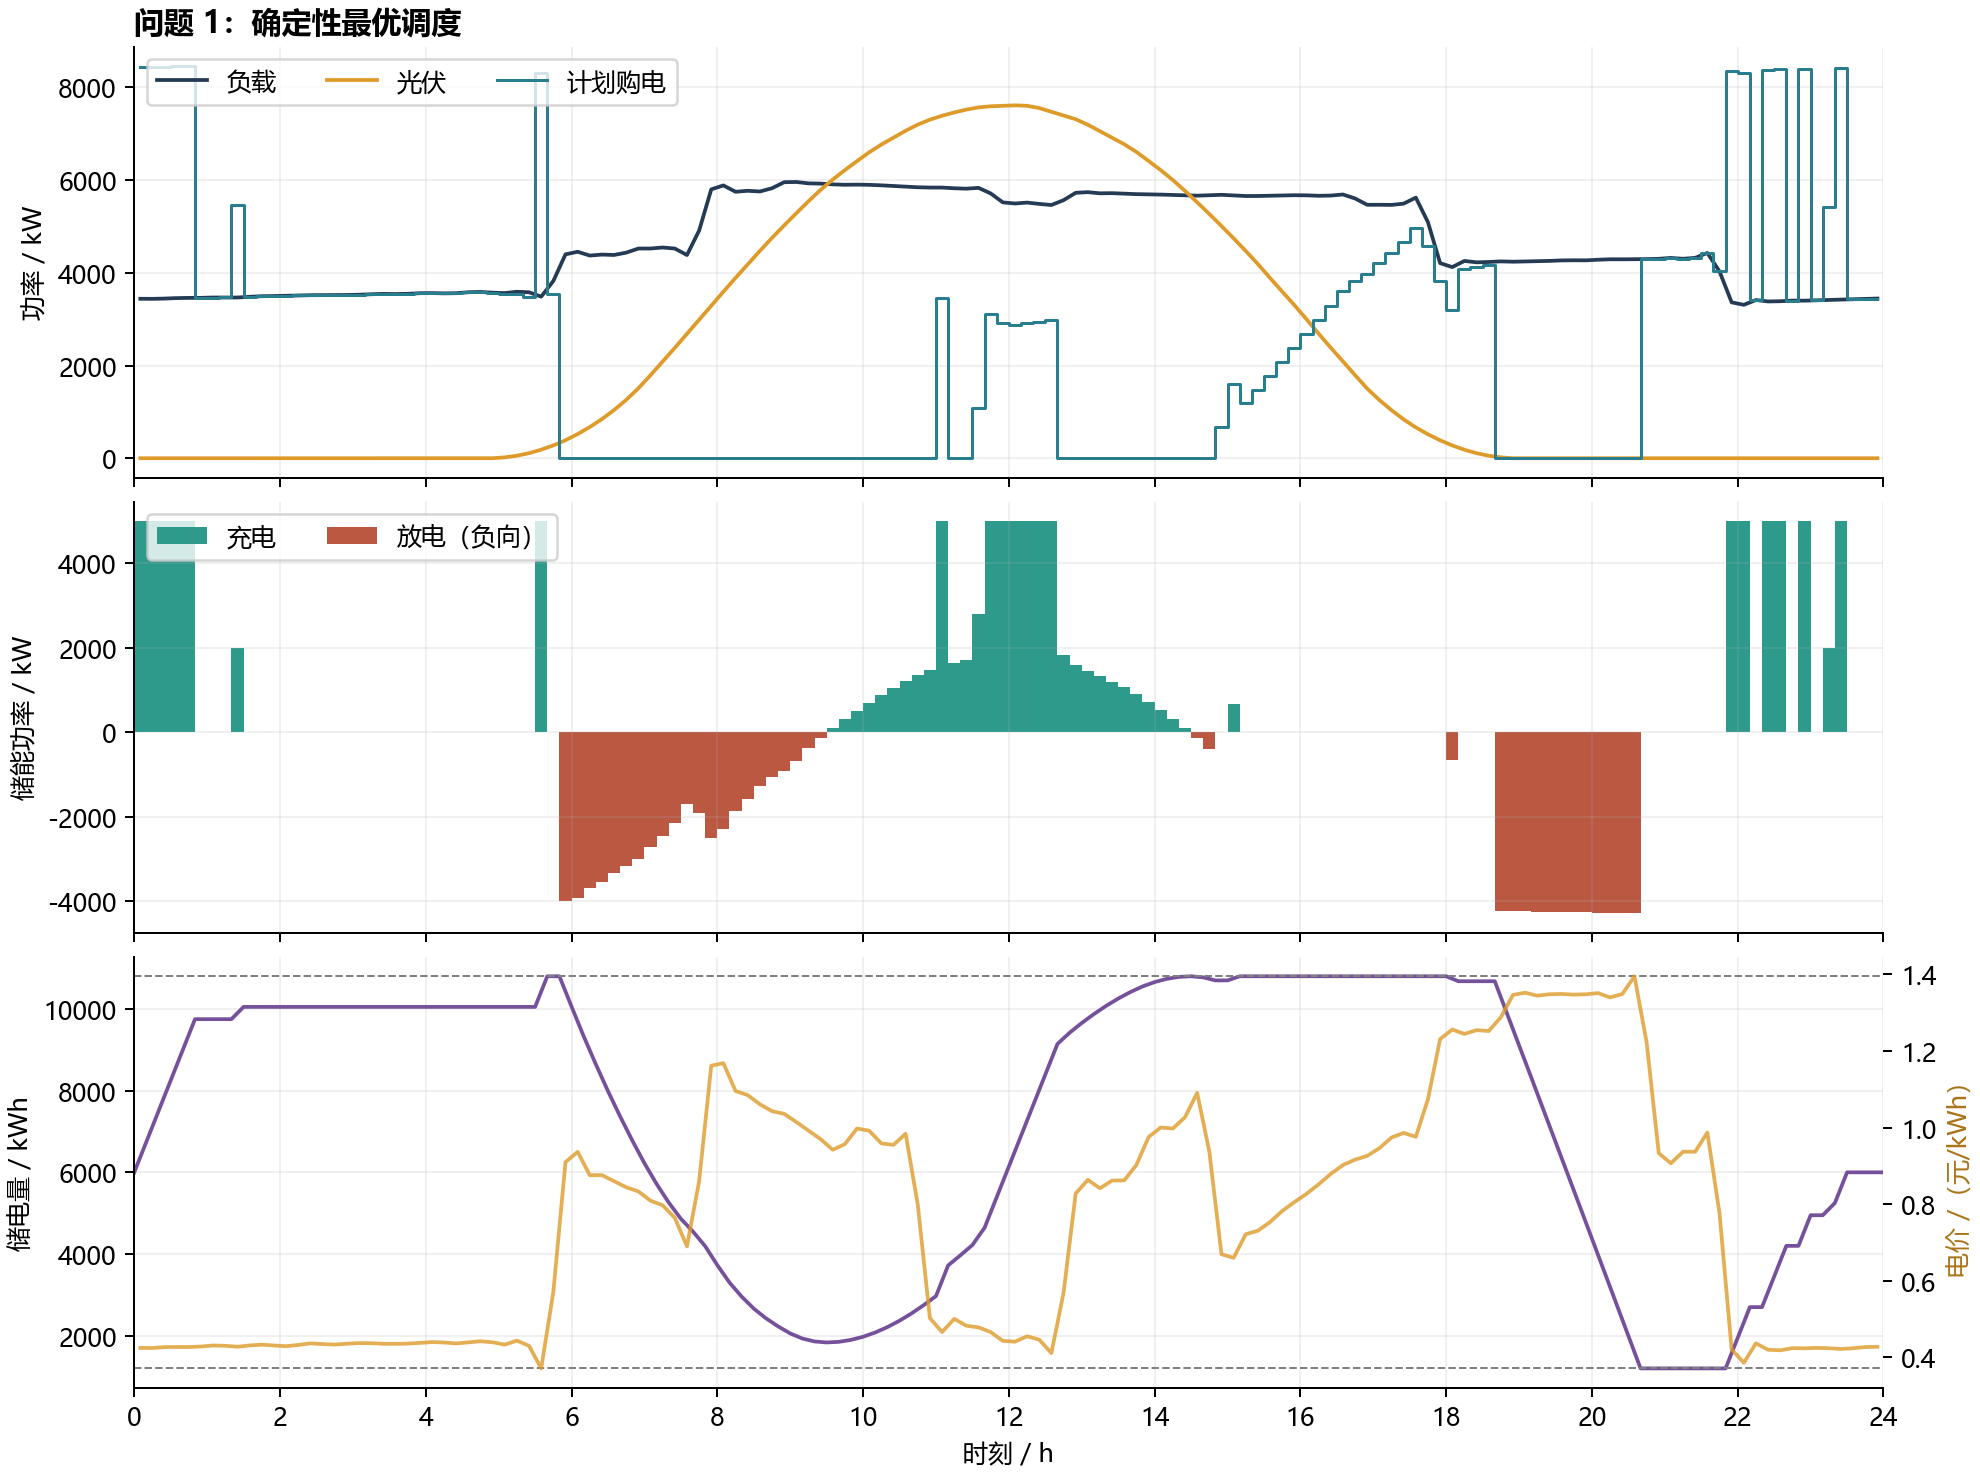
\includegraphics[width=\textwidth]{../outputs/figures/q1-dispatch.png}
  \caption{问题一的最优购电与储能调度}\label{fig:q1}
\end{figure}
在低电价或光伏富余区间储能，可在高电价时替代购电。但每向电池输入1\,kWh，只能最终向母线输出0.81\,kWh；仅考虑套利时，放电段替代电价至少要高于充电段电价除以0.81。容量和功率约束进一步限制了负荷可以转移的数量。表中某个四小时区间内充电总量与放电总量同时为正，并不意味着某个十分钟段同时充放电。
\FloatBarrier

\clearpage
\subsection{问题二：历史预测、风险计划与实时执行}
\subsubsection{历史负荷与光伏预测}
设$P^L_{d,t},P^V_{d,t}$为功率观测。对具有至少一周历史的日期，负荷的同星期预测为
\begin{equation}
 \widehat P^L_{d,t}=\frac{\sum_{k=1}^{K_d}0.55^{k-1}P^L_{d-7k,t}}
 {\sum_{k=1}^{K_d}0.55^{k-1}},\qquad K_d=\min\{4,\lfloor d/7\rfloor\}.
\end{equation}
日期索引从1月1日的$d=0$开始。历史不足7天时，改用此前最多7天同刻值，以$0.8^{k-1}$加权。光伏采用较短窗口：
\begin{equation}
 \widehat P^{V,H}_{d,t}=\frac{\sum_{k=1}^{\min(7,d)}0.75^{k-1}P^V_{d-k,t}}
 {\sum_{k=1}^{\min(7,d)}0.75^{k-1}}.
\end{equation}
无历史的首日负荷先验为4500\,kW、光伏为0，仅用于1月初始运行。两类预测均只读取日期$d$之前的观测，不把附件一包含全年信息的典型曲线作为先验。净负荷电量点预测为
\begin{equation}
 \widehat N_{d,t}=\Delta(\widehat P^L_{d,t}-\widehat P^{V,H}_{d,t}),\qquad\Delta=1/6\ \mathrm{h}.
\end{equation}

\subsubsection{经验风险分位与零时计划}
直接按点预测购电会低估紧急购电的非对称代价。对预测发布时刻$r$，保存其对应预测器的历史残差
\begin{equation}
 R^{(r)}_{j,t}=N_{j,t}-\widehat N^{(r)}_{j,t}.
\end{equation}
仅使用$\max(7,d-28)\le j<d$的日期，将同刻及前后各3个十分钟段的残差合并；在当前发布时刻至日末的剩余预测区间两端，按端点复制补齐邻域。由所得集合$\mathcal R^{(r)}_{d,t}$形成风险调整量
\begin{equation}
 \widetilde N^{(r)}_{d,t}=\widehat N^{(r)}_{d,t}
   +Q_{\alpha}\!\left(\mathcal R^{(r)}_{d,t}\right).\label{eq:risk}
\end{equation}
经验分位对排序样本采用线性插值，即NumPy的\texttt{quantile}默认规则。没有足够历史时不添加分位修正。不同光伏融合权重或信息子集各自重算历史预测与残差，避免混用预测器的误差分布。

零时读取上一日真实末库存，在当日144段上将式\eqref{eq:balance}的净负荷换成$\widetilde N$、令$e_t=0$，最小化预测常规购电费，增加$S_{144}\ge6000$的规划约束。由此生成固定原计划$g_t$。分位参数越大，通常越倾向于提前购入电量，但可能产生更多付费余电；费用随参数未必单调，且电池把各时段连接起来，不能把单段分位直接解释为全系统的供电可靠性保证。

已有两阶段微网调度研究将日前储能SOC下限传入日内决策，并联合考虑应急供能成本\cite{hu2025emergency}，说明库存管理与应急支出需要协调。本文的6000\,kWh是自行设定的日末规划恢复目标，并非从该文推得的最优下限，也不涉及其应急电源车决策。

候选分位为$\{0.50,0.65,0.70,0.80,0.90,0.95\}$，按1月15日至31日的实际现金支出选择；候选从1月1日6000\,kWh起以自身固定参数回放。问题二选择$\alpha=0.80$。正式策略的1月热启动固定使用0.80分位，随后连续承接库存，2—12月计入正式结果。

\subsubsection{十分钟安全反馈与费用}
令$z_t=q_t-(L_t-V_t)$表示常规电力相对实际净需求的余量。在每个交付段观察到实际需求后，采用
\begin{align}
 z_t\ge0:&\quad c_t=\min\{z_t,5000/6,(10800-S_t)/0.9\},\quad b_t=e_t=0,\quad w_t=z_t-c_t;\\
 z_t<0:&\quad b_t=\min\{-z_t,5000/6,0.9(S_t-1200)\},\quad c_t=w_t=0,\quad e_t=-z_t-b_t.
\end{align}
每步按式\eqref{eq:soc}更新库存。无外网紧急购电上限时，$e_t$消除剩余缺口，保证物理可行；它不会被用于额外给电池充电。问题二的实际账单为
\begin{equation}
 C_2=\sum_{d,t}\left(p_tg_{d,t}+5p_te_{d,t}\right).
\end{equation}
该反馈在缺口出现时尽量放电，是简单、可复现的可行控制。它没有比较跨时段紧急电价，也没有评估储存1\,kWh电能的未来价值，因此不能由可行性推导经济最优性。第\ref{sec:feedback}节另给价格感知反馈对照。

\clearpage
\subsection{问题三：日内调整购电规划}\label{sec:q3}
\subsubsection{新增信息与交易变量}
问题三在固定电价下，每天00、06、12、18点可获得未来整点的光伏预报，并可在后三个时刻修订尚未交付的购电量。新预报有助于更新对光伏出力的判断，日内调整则可以结合实际库存和近期负荷重新安排购电。为判断两者各自的作用，后文在相同调整时刻下比较不同预报的使用效果。

记零时计划为$g_{d,t}$，发布时间对应的区间索引为$s\in\{0,36,72,108\}$，在$s$修订的剩余计划为$q^{(s)}_{d,t}$，最终交付的常规电量为$q_{d,t}$。规划根据预测安排购电，运行时仍按问题二的规则调节储能。可用信息$\mathcal H_{d,s}$包括此前日期的历史、当日$s$之前已完成区间的观测，以及截至$s$已发布的预报。

本问沿用余电可以不利用、原计划款不返还的假设。主要计算按每段最终交付量与零时计划的差额收费，允许撤回尚未交付的追加申报。下文将这一解释称为主合约，另比较追加电量成交后不可撤回、每笔分别收费的情形。

\subsubsection{费用目标与预报融合}
总费用由原计划、调整和紧急购电三项组成：
\begin{equation}
\begin{aligned}[b]
 C_3=\sum_{d,t}\bigl[&p_tg_{d,t}
 +1.5p_t(q_{d,t}-g_{d,t})_+\\
 &+0.5p_t(g_{d,t}-q_{d,t})_+
 +5p_te_{d,t}\bigr].
\end{aligned}\label{eq:netbill}
\end{equation}
其中$(x)_+=\max(x,0)$，求和覆盖正式期。增购1\,kWh额外支付$1.5p_t$；减购1\,kWh时，原计划款照付，另加$0.5p_t$违约费，即原价的50\%。

零时按$(\mathrm P_2)$制定计划，净负荷预测采用已发布预报与历史数据的融合结果。日内$s>0$时，原计划费用已经确定，因此重新规划以剩余时段的增购费用最小为目标：
\begin{equation}
 \min \widehat C_{3,d,s}=\sum_{t=s}^{143}1.5p_t\bigl(q^{(s)}_{d,t}-g_{d,t}\bigr).\label{eq:replan}
\end{equation}
本式采用$q^{(s)}_{d,t}\ge g_{d,t}$的约束，理由见下节。与问题二相同，未来紧急购电的风险通过净负荷分位修正来处理，实际费用则在运行后核算。

附件三中，$h$点发布的第$k$列预报对应$h+k$点。每次收到预报后，以最近一个已完成区间的光伏观测为插值起点，依次连接未来整点值，得到十分钟预测$\widehat P^{\mathrm{V,F}}$，并取其中截至当日24点的部分。

采用两来源线性融合：
\begin{equation}
 \widehat P^{\mathrm V}_{d,t}
 =(1-\lambda)\widehat P^{\mathrm{V,H}}_{d,t}
 +\lambda\widehat P^{\mathrm{V,F}}_{d,t},
 \qquad 0\le\lambda\le1.\label{eq:fusion}
\end{equation}
不同来源的预测误差可能相互补充，因而可通过组合改善预测\upcite{bates1969combination}，光伏预测中也已有自适应组合的研究\upcite{wei2026pv}。本文采用上述加权形式，并按实际购电费用选择权重，使预测效果能够通过最终支出评价。

为避免近期观测使预测水平发生过大跳变，先定义区间截断函数：
\begin{equation}
 \operatorname{clip}(x,a,b)=\min\{b,\max\{a,x\}\},\qquad a\le b.\label{eq:clip}
\end{equation}
其中$x$为待修正的数值，$a$、$b$分别为下限和上限：小于$a$时返回$a$，大于$b$时返回$b$，在区间内则保留$x$。本文将它作用于无量纲修正比例，例如$\operatorname{clip}(1.40,0.75,1.25)=1.25$。

在日内发布时刻$s\in\{36,72,108\}$，再用此前18个已完成区间，即最近3小时的观测修正负荷水平：
\begin{equation}
 \widehat P^{\mathrm L,(s)}_{d,t}
 =\widehat P^{\mathrm L}_{d,t}
 \operatorname{clip}\!\left(
 \frac{\overline{P^{\mathrm L}_{d,s-18:s}}}
      {\max(\overline{\widehat P^{\mathrm L}_{d,s-18:s}},1)},0.75,1.25
 \right),\quad t\ge s.
\end{equation}
横线表示索引$j=s-18,\ldots,s-1$上的算术均值，分母中的1以kW计，用于避免预测均值过小导致比值异常。该比值反映最近实际负荷与原预测的偏差。按式\eqref{eq:clip}限制在$[0.75,1.25]$后，每次修正幅度至多为原预测的25\%；上下限由控制规则设定，未作置信水平解释。将修正后的负荷与融合光伏相减，形成净负荷点预测，再按式\eqref{eq:risk}加入对应发布时间的历史残差分位。每种$\lambda$和预报组合分别计算残差，所用样本均来自此前日期。

\subsubsection{分条约束与汇总模型}
\textbf{a) 剩余时域供需平衡。}仅对$t\ge s$规划未来交付：
\begin{equation}
 q^{(s)}_{d,t}+\widehat b_{d,t}
 =\widetilde N^{(s)}_{d,t}+\widehat c_{d,t}+\widehat w_{d,t}.
\end{equation}
已交付区间不重新优化，其实际费用和库存变化均保留。

\textbf{b) 实际库存起点。}每次规划采用当时实际储电量，即$\widehat S_{d,s}=S_{d,s}$，并要求$\widehat S_{d,144}\ge6000$。预测中的储能运行继续满足问题一的状态递推、功率和库存限制。

\textbf{c) 原计划下界。}若某段$q<g$，可将$q$提高到$g$，差额计入未利用量。此时充放电和库存相同，还可省去减购违约费。因此，按主合约保留原计划量的费用更低，可加入
\begin{equation}
 q^{(s)}_{d,t}\ge g_{d,t},\qquad t\ge s.\label{eq:plan-floor}
\end{equation}
各次修订均以零时$g_t$为下界。此前的$q^{(s-36)}_t$中尚未交付的追加量可以撤回，费用最终按交付量与原计划的净差计算。

\textbf{d) 信息与动作时点。}本次$q^{(s)}$根据$\mathcal H_{d,s}$制定；此后各交付段获得的实际需求用于充放电反馈和紧急补购，已交付电量按当时计划记录。

省略日期下标，得到每次日内重规划的完整形式：
\begin{equation}
\begin{aligned}[b]
 (\mathrm P_3^{(s)})\quad\min\quad&
       \sum_{t=s}^{143}1.5p_t(q^{(s)}_t-g_t),\\
 \mathrm{s.t.}\quad&q^{(s)}_t+\widehat b_t
      =\widetilde N^{(s)}_t+\widehat c_t+\widehat w_t,\\
 &\widehat S_{t+1}=\widehat S_t+0.9\widehat c_t-\widehat b_t/0.9,\\
 &0\le\widehat c_t,\widehat b_t\le5000/6,\quad\widehat w_t\ge0,\quad q^{(s)}_t\ge g_t,\\
 &1200\le\widehat S_t\le10800,\quad
   \widehat S_s=S_{d,s},\quad\widehat S_{144}\ge6000.
\end{aligned}\label{eq:q3-summary}
\end{equation}
区间约束作用于$t=s,\ldots,143$，库存边界还包括144。剩余时域分别为108、72、36段，相应线性规划为540、360、180个连续变量。充放电互斥仍可按问题一的论证处理。

\subsubsection{求解与日内执行步骤}
权重候选为$\{0,0.25,0.50,0.75,1\}$，与六个分位组成30组参数。按1月15—31日实际费用比较，选得$(\lambda,\alpha)=(0.50,0.65)$。正式运行采用的1月热启动预先固定为纯附件三预测、0.80分位及三次日内调整，2月1日起使用所选参数。候选模拟仅用于评分，正式策略的初始库存由预先固定的热启动运行确定。

日前与日内协调优化已有相关研究\upcite{xiao2019mpc}。本问采用如下分时执行步骤：
\begin{enumerate}
 \item 零时继承真实库存，读取已发布光伏预报，与历史曲线融合并作风险修正，求解全天原计划$g$。
 \item 每到06、12、18点，接收本次新预报和此前已完成区间的负荷、光伏观测，更新剩余预测。
 \item 以当前实际库存为起点，求解$(\mathrm P_3^{(s)})$，更新尚未交付的常规计划，并记录各次修订。
 \item 在每个交付段以当前$q_t$替换问题二反馈式中的$g_t$，执行储能和必要的紧急购电。
 \item 根据最终$q_t-g_t$计算主合约调整费，日末将实际库存传至次日。
\end{enumerate}
日内LP给出当次预测下费用最低的常规计划，后续效果还取决于实际需求和储能反馈。因此，本问得到的是基于预测的可行调度策略。

\subsubsection{调度结果与费用来源}
正式期总费用为\PaperValue{q3-cost}\,元，比问题二减少\PaperValue{q3-saving}\,元，降幅\PaperValue{q3-saving-percent}\%。表\ref{tab:q3-comparison}将费用、电量和库存放在同一口径下比较。
\par
\begin{table}[!htbp]
\centering
\caption{固定电价下两种策略的结果（2—12月）}\label{tab:q3-comparison}
\normalsize
\begin{tabular}{lrr}
\toprule
\multicolumn{1}{c}{指标} & \multicolumn{1}{c}{零时固定计划} & \multicolumn{1}{c}{日内调整计划} \\
\midrule
原计划费/元 & 13,291,625.72 & 12,649,467.17 \\
调整费/元 & 0.00 & 527,937.93 \\
紧急费/元 & 616,550.23 & 138,430.89 \\
总费用/元 & 13,908,175.95 & 13,315,835.99 \\
常规购电/kWh & 21,712,548.31 & 21,197,074.02 \\
紧急购电/kWh & 102,787.48 & 25,862.57 \\
未利用电量/kWh & 2,646,069.43 & 2,021,445.81 \\
发生紧急购电的天数 & 115 & 139 \\
期初储电量/kWh & 6,840.33 & 7,089.87 \\
期末储电量/kWh & 6,258.37 & 5,987.72 \\
\bottomrule
\end{tabular}
\end{table}
\par

\FloatBarrier
原计划费由13291625.72元降至12649467.17元，紧急费由616550.23元降至138430.89元，两项节省超过了新增的527937.93元调整费。常规购电量和未利用电量也有所下降，日内方案通过重新安排购电数量和时段，减少了提前多购与高价补购的支出。

紧急购电总量下降约74.84\%，发生天数却从115天增至139天，说明日内方案降低了紧急电量及支出，发生频率仍需关注。两种主策略的热启动不同，表中同时列出首末库存；费用差反映各自连续运行的实际支出。

表\ref{tab:q3-days-summary}汇总四个指定日期，正文按题面格式列出9月23日，其他日期及紧急事件、账单见附录\ref{app:q3-days}，与\texttt{result3.xlsx}对应。购电表用相同的六列结构分别展示零时原计划和最终常规购电，两者之差才是净调整量。原计划部分的“全天购电费”为原计划费，最终部分为原计划费加调整费，均不含紧急费；储能表为实际执行值。
\par
\begin{table}[!htbp]
\centering
\caption{问题三的指定日期结果（2025年）}\label{tab:q3-days-summary}
\normalsize
\begin{tabular}{lrrr}
\toprule
\multicolumn{1}{c}{日期} & \multicolumn{1}{c}{常规购电/kWh} & \multicolumn{1}{c}{紧急购电/kWh} & \multicolumn{1}{c}{全天总费用/元} \\
\midrule
03-20 & 67,646.32 & 0.00 & 41,647.19 \\
06-21 & 35,854.93 & 0.00 & 20,909.49 \\
09-23 & 67,230.48 & 170.85 & 43,904.67 \\
12-21 & 96,803.32 & 0.00 & 62,129.52 \\
\bottomrule
\end{tabular}
\end{table}
\par

% Generated by scripts/build_paper_tables.py; do not edit by hand.
2025.9.23的购电和储能结果分别见表\ref{tab:q3-2025-09-23-purchase}和表\ref{tab:q3-2025-09-23-storage}。

\par
\begin{table}[!htbp]
\centering
\caption{微网在指定时间段的购电量及全天的购电量和购电费（2025.9.23）}\label{tab:q3-2025-09-23-purchase}
\normalsize
\begin{tabular}{lrlrlr}
\toprule
\multicolumn{6}{c}{零时原计划} \\
\multicolumn{1}{c}{时间段} & \multicolumn{1}{c}{购电量} & \multicolumn{1}{c}{时间段} & \multicolumn{1}{c}{购电量} & \multicolumn{1}{c}{时间段} & \multicolumn{1}{c}{购电量} \\
\midrule
10:00--10:10 & 0.00 & 12:00--12:10 & 401.83 & 14:00--14:10 & 0.00 \\
16:00--16:10 & 520.87 & 18:00--18:10 & 763.88 & 20:00--20:10 & 0.00 \\
\multicolumn{2}{c}{全天购电量} & 65,285.63 & \multicolumn{2}{c}{全天购电费} & 40,305.24 \\
\addlinespace
\multicolumn{6}{c}{最终常规购电} \\
时间段 & 购电量 & 时间段 & 购电量 & 时间段 & 购电量 \\
10:00--10:10 & 0.00 & 12:00--12:10 & 401.83 & 14:00--14:10 & 0.00 \\
16:00--16:10 & 520.87 & 18:00--18:10 & 793.71 & 20:00--20:10 & 0.00 \\
\multicolumn{2}{c}{全天购电量} & 67,230.48 & \multicolumn{2}{c}{全天购电费} & 43,084.92 \\
\bottomrule
\end{tabular}
\end{table}
\par


\par
\begin{table}[!htbp]
\centering
\caption{储能设备在指定时间段的充放电量及0:00和24:00的储电量（2025.9.23）}\label{tab:q3-2025-09-23-storage}
\normalsize
\begin{tabular}{lrrlrr}
\toprule
\multicolumn{1}{c}{时间段} & \multicolumn{1}{c}{充电量} & \multicolumn{1}{c}{放电量} & \multicolumn{1}{c}{时间段} & \multicolumn{1}{c}{充电量} & \multicolumn{1}{c}{放电量} \\
\midrule
0:00--4:00 & 4,254.93 & 310.26 & 4:00--8:00 & 1,030.38 & 6,166.49 \\
8:00--12:00 & 5,281.76 & 1,896.62 & 12:00--16:00 & 5,321.25 & 534.56 \\
16:00--20:00 & 111.95 & 5,842.00 & 20:00--24:00 & 5,560.36 & 2,696.82 \\
\multicolumn{2}{c}{0:00储电量} & 6,177.67 & \multicolumn{2}{c}{24:00储电量} & 6,196.96 \\
\bottomrule
\end{tabular}
\end{table}
\par


\FloatBarrier
9月23日紧急电量从问题二的892.40\,kWh降至170.85\,kWh，总费下降3909.92元；3月20日日内方案却比问题二多支出109.40元，说明调整机会并不保证每一天都降低费用。
图\ref{fig:q3-day}展示9月23日的原计划、最终购电与实际净需求；竖虚线标出三次允许修订的时刻。最终购电在原计划上补充部分缺口，后续库存因此改变，紧急购电的规模随之下降。
\begin{figure}[!htbp]
 \centering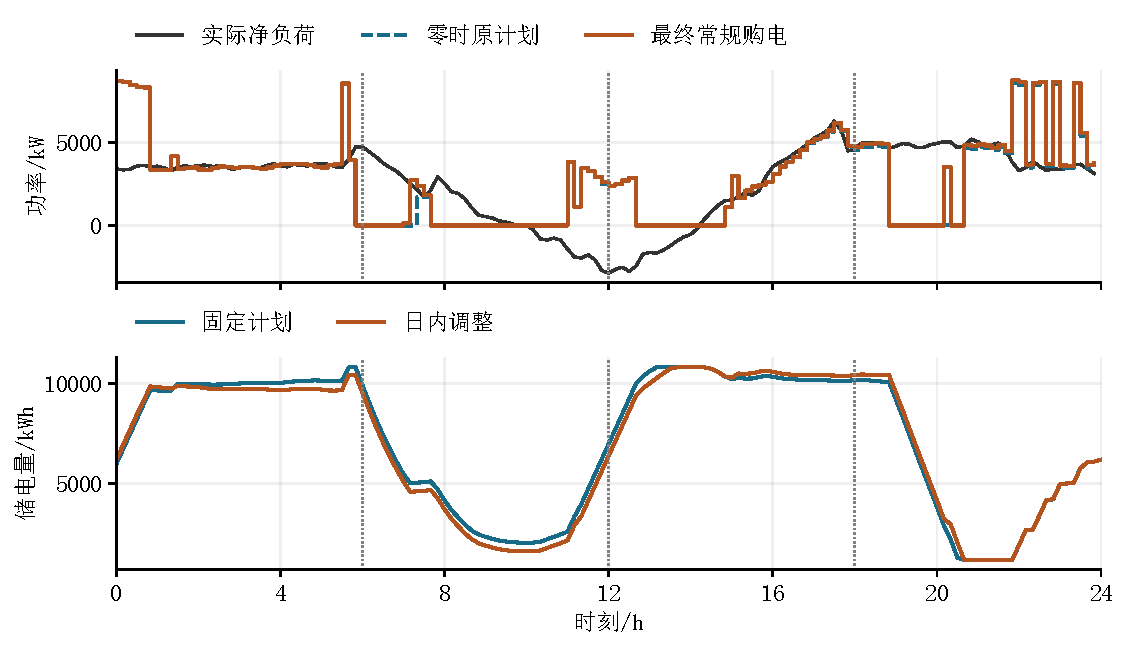
\includegraphics[width=\textwidth]{../outputs/figures/paper-q3-day.pdf}
 \caption{9月23日的日内购电调整与库存变化}\label{fig:q3-day}
\end{figure}
\FloatBarrier

\subsubsection{预报贡献与参数灵敏度}
各光伏来源先在相同1月区间选参，再从共同热启动和期初库存开始比较。融合方案比纯历史基准节省112379.91元，单用附件三则更贵，说明保留历史预测有助于降低本题的运行费用。完整费用见附录\ref{app:parameter-checks}表\ref{tab:q3-forecast}。某次新预报的作用，还需进一步控制调整机会等条件。

为判断是否需要其他时刻的预报，各组采用相同主参数、三次调整时刻、负荷修正及光伏插值起点，逐组改变允许读取的新预报；不读取时沿用最近可用的一次。各组共用1月热启动，随后按自身调度连续运行。表\ref{tab:hourly-marginals}列出每次单独撤去一项预报后的费用变化，八种组合的完整结果见附录\ref{app:parameter-checks}表\ref{tab:hourly-subsets}。
% Generated by scripts/build_paper_tables.py; do not edit by hand.
\par
\begin{table}[!htbp]
\centering
\caption{单独撤去一次新小时预报的条件费用差（元）}\label{tab:hourly-marginals}
\normalsize
\begin{tabular}{lrr}
\toprule
\multicolumn{1}{c}{撤去的预报} & \multicolumn{1}{c}{纯附件3} & \multicolumn{1}{c}{融合主策略} \\
\midrule
06点 & 53,593.3113 & 28,402.5518 \\
12点 & 74,628.9683 & 20,127.5241 \\
18点 & -0.1296 & -0.3123 \\
\bottomrule
\end{tabular}
\end{table}
\par

\FloatBarrier
读取全部新预报比均不读取节省17225.82元。撤去06或12点的新预报会增加费用，撤去18点后的变化仅$-0.31$元。因此，在本组参数下，前两次新预报有助于降低费用，18点的新预报收益很小。各次预报的影响随库存和后续计划相互关联，单项费用差不能直接相加。对照仍保留18点调整，可利用当时的负荷观测和库存变化重新安排购电。

分位扰动见表\ref{tab:q3-risk-sensitivity}。正式期$\alpha=0.50$的费用比主参数0.65低15787.50元，但紧急电量明显增大。1月评分较低的参数未必在后续月份同样省费，短期选参存在样本局限。主结果采用按1月费用选出的参数，全年扰动用于考察这一选择的影响。
\par
\begin{table}[!htbp]
\centering
\caption{问题三的分位参数扰动（2—12月）}\label{tab:q3-risk-sensitivity}
\normalsize
\begin{tabular}{lrrr}
\toprule
\multicolumn{1}{c}{$\alpha$} & \multicolumn{1}{c}{总费用/元} & \multicolumn{1}{c}{紧急购电/kWh} & \multicolumn{1}{c}{年末储电量/kWh} \\
\midrule
0.5 & 13,300,048.49 & 66,633.50 & 5,890.36 \\
0.65 & 13,315,835.99 & 25,862.57 & 5,987.72 \\
0.7 & 13,393,753.32 & 18,804.41 & 6,060.07 \\
0.9 & 14,101,446.70 & 2,544.90 & 6,507.64 \\
\bottomrule
\end{tabular}
\end{table}
\par

将日末预测恢复目标改为3000或9000\,kWh，结果见附录\ref{app:parameter-checks}表\ref{tab:q3-reserve}。目标较低时支出下降，热启动库存和期末库存也随之降低，因此费用变化同时反映了购电安排和储备电量的差异。
\FloatBarrier
逐笔成交不可撤回时，重新选参和优化的总费为\PaperValue{q3-per-trade-cost}\,元，仍比问题二低447673.33元，但节省少于主合约。附录\ref{sec:contracts}分别给出原调度重新计费及重新优化的结果，说明累计调整费的规则会影响方案收益。
\label{end:q3}

\clearpage
\subsection{问题四：波动电价下的规划}\label{sec:q4}
\subsubsection{价格信息与两种决策频率}
问题四采用附件四的实时波动电价。价格变化会影响哪些时段适合购电和储能，因此需要根据预测价格重新制定计划，再按实际价格计算支出。未来电价在决策时尚未知晓，预测控制与预先知道全部价格时的表现存在差别，相关动态价格研究也讨论了这一问题\upcite{perez2023hem}。

本文将“交易时刻电价”解释为对应交付区间的实际价格$p_{d,t}$，用于交付结算。沿用问题三的交易变量，记$\widehat p^{(s)}_{d,t}$为时刻$s$基于已有信息预测的未来电价。问题4-2在$s=0$制定全天固定计划；问题4-3在$s\in\{0,36,72,108\}$进行滚动规划，并沿用光伏预报融合及最终净调整合约。

两种策略采用相同的设备参数、十分钟步长及储能反馈规则，实际储电量均随每日运行连续传递。

\subsubsection{费用目标与价格预测}
问题4-2和4-3的实际购电费用分别为
\begin{equation}
 C_{4-2}=\sum_{d,t}p_{d,t}(g_{d,t}+5e_{d,t}),
\end{equation}
\begin{equation}
\begin{aligned}[b]
 C_{4-3}=\sum_{d,t}p_{d,t}\bigl[&g_{d,t}
 +1.5(q_{d,t}-g_{d,t})_+\\
 &+0.5(g_{d,t}-q_{d,t})_++5e_{d,t}\bigr].
\end{aligned}\label{eq:q4-bill}
\end{equation}
费用均统计2—12月，并按实际价格计算。制定计划时，用预测价格代替尚未知晓的未来价格，零时和日内分别求解
\begin{equation}
 \min\sum_{t=0}^{143}\widehat p^{(0)}_{d,t}g_{d,t},
 \qquad
 \min\sum_{t=s}^{143}1.5\widehat p^{(s)}_{d,t}
       (q^{(s)}_{d,t}-g_{d,t}).\label{eq:q4-objectives}
\end{equation}
第二个目标用于问题4-3的$s>0$。两项目标决定当次购电安排，最终费用则由实际交付电量和价格核算。

电价预测考虑周周期特征。当$d\ge7$时，选取此前最多四个与目标日星期相同的日期，对同一时刻电价进行衰减加权：
\begin{equation}
 \overline p_{d,t}=
 \frac{\sum_{k=1}^{K_d}0.55^{k-1}p_{d-7k,t}}
      {\sum_{k=1}^{K_d}0.55^{k-1}},
 \qquad K_d=\min\{4,\lfloor d/7\rfloor\}.
\end{equation}
历史不足一周时，取此前最多7天，以0.8的衰减系数加权。零时取$\widehat p^{(0)}_{d,t}=\max(\overline p_{d,t},0.001)$。问题4-3在日内根据最近18段实际价格的均值修正预测水平，使用式\eqref{eq:clip}将修正比例限制在$[0.5,1.5]$。记
\begin{equation}
 r^{p}_{d,s}=\operatorname{clip}\!\left(
 \frac{\frac1{18}\sum_{j=s-18}^{s-1}p_{d,j}}
      {\max\left(\frac1{18}\sum_{j=s-18}^{s-1}\overline p_{d,j},0.01\right)},
 0.5,1.5\right),
\end{equation}
由此得到剩余时段的价格预测：
\begin{equation}
 \widehat p^{(s)}_{d,t}=\max\{0.001,r^{p}_{d,s}\overline p_{d,t}\},
 \qquad t\ge s,\quad d\ge1.\label{eq:price-update}
\end{equation}
比例截断可避免历史均值很小时产生过大的修正，价格下限保证目标系数为正。首日各发布时间均采用附件一的固定价格，用于1月初始化；从随后日期起，按已完成区间的观测计算预测和修正比例。

\subsubsection{分条约束与汇总模型}
\textbf{a) 物理约束。}每次规划仍满足风险净负荷下的能量平衡、储能效率、功率和安全库存限制。价格改变目标系数，不改变物理守恒关系。

\textbf{b) 库存衔接。}零时从实际$S_{d,0}$开始，日内从实际$S_{d,s}$开始，预测日末恢复目标均为6000\,kWh。实际跨日运行不重置库存。

\textbf{c) 交易频率与原计划下界。}问题4-2全天$q_t=g_t$；问题4-3在三次允许时刻修改未交付量，且$q^{(s)}_t\ge g_t$。实际和预测价格均为正，故问题三关于保留原计划量更有利的论证仍适用。

\textbf{d) 可用信息与实际结算。}预测价格、净负荷和本次计划均由$\mathcal H_{d,s}$确定；之后观测到的$p_{d,t}$用于结算对应交付段的费用，已执行决策保留原记录。

为统一两种频率，令允许的发布时间集合为$\mathcal S$；零时取$\ell^{(0)}_t=0$、$\kappa_0=1$，日内取$\ell^{(s)}_t=g_t$、$\kappa_s=1.5$。每次求解
\begin{equation}
\begin{aligned}[b]
 (\mathrm P_4^{(s)})\quad\min\quad&
  \sum_{t=s}^{143}\kappa_s\widehat p^{(s)}_{d,t}
       (q^{(s)}_t-\ell^{(s)}_t),\\
 \mathrm{s.t.}\quad&q^{(s)}_t+\widehat b_t
       =\widetilde N^{(s)}_{d,t}+\widehat c_t+\widehat w_t,\\
 &\widehat S_{t+1}=\widehat S_t+0.9\widehat c_t-\widehat b_t/0.9,\\
 &0\le\widehat c_t,\widehat b_t\le5000/6,\quad
   q^{(s)}_t\ge\ell^{(s)}_t,\quad\widehat w_t\ge0,\\
 &1200\le\widehat S_t\le10800,\quad
   \widehat S_s=S_{d,s},\quad\widehat S_{144}\ge6000.
\end{aligned}\label{eq:q4-summary}
\end{equation}
零时求得的计划为$g_t=q^{(0)}_t$。问题4-2取$\mathcal S=\{0\}$，问题4-3取$\mathcal S=\{0,36,72,108\}$；区间约束作用于$t=s,\ldots,143$，库存边界还包括144。模型据此统一表示两种规划频率。

\subsubsection{求解与结算步骤}
沿用问题二、三的候选集合，按1月15—31日实际费用选参。问题4-2选得$\alpha=0.80$，问题4-3选得$(\lambda,\alpha)=(0.50,0.65)$。问题4-3的1月热启动固定使用纯附件三预测、0.80分位及三次调整，2月起采用所选参数。

按时间先后运行以下步骤：
\begin{enumerate}
 \item 零时继承真实库存，以过去日期分别预测负荷、光伏和价格；构造风险净负荷。
 \item 用预测价格作为目标系数求解$(\mathrm P_4^{(0)})$，锁定原计划并保存预测曲线。
 \item 问题4-2按固定计划运行；问题4-3在各发布时间利用新预报及最近观测更新负荷、光伏和价格预测，求解剩余时段模型。
 \item 交付时根据当段实际净负荷执行充放电，放电后的缺口由紧急购电补足。
 \item 用该段实际价格结算原计划、最终净调整和紧急购电，更新实际库存。
 \item 日末传递库存，2月起累计正式费用；从逐段数组分别重算全年和指定日期账单。
\end{enumerate}

为检查信息使用顺序，将未来实际价格替换后重新计算，确认当前预测和计划不受影响。历史误差也按日期和发布时间读取，只有已完成区间的误差参与当前修正。

\subsubsection{波动电价结果及比较}
问题4-2总费用为\PaperValue{q4-2-cost}\,元，问题4-3为\PaperValue{q4-3-cost}\,元，日内方案节省\PaperValue{q4-3-saving}\,元，降幅\PaperValue{q4-3-saving-percent}\%。表\ref{tab:q4-comparison}给出费用与电量分解。
\par
\begin{table}[!htbp]
\centering
\caption{波动电价下两种策略的结果（2—12月）}\label{tab:q4-comparison}
\normalsize
\begin{tabular}{lrr}
\toprule
\multicolumn{1}{c}{指标} & \multicolumn{1}{c}{问题4-2} & \multicolumn{1}{c}{问题4-3} \\
\midrule
原计划费/元 & 14,032,328.84 & 13,366,608.69 \\
调整费/元 & 0.00 & 550,605.94 \\
紧急费/元 & 643,516.03 & 127,670.62 \\
总费用/元 & 14,675,844.87 & 14,044,885.25 \\
常规购电/kWh & 21,708,087.29 & 21,192,613.91 \\
紧急购电/kWh & 101,425.76 & 24,227.41 \\
未利用电量/kWh & 2,632,806.82 & 2,009,834.69 \\
发生紧急购电的天数 & 108 & 134 \\
期初储电量/kWh & 6,864.27 & 7,114.54 \\
期末储电量/kWh & 6,263.02 & 5,997.11 \\
\bottomrule
\end{tabular}
\end{table}
\par

\FloatBarrier
日内方案降低了原计划费和紧急费，计入新增550605.94元调整费后，总支出仍较低。紧急电量由101425.76\,kWh降至24227.41\,kWh，发生天数却由108增至134。与固定电价下相同，紧急购电的总规模缩小，但分布在更多日期。

图\ref{fig:q4-months}给出逐月费用及紧急电量，便于在相同月份和实际电价下比较两种策略。固定电价与波动电价的费用差还包含价格水平、购电安排和库存变化，解释这一差异时需同时考虑这些因素。
\begin{figure}[!htbp]
 \centering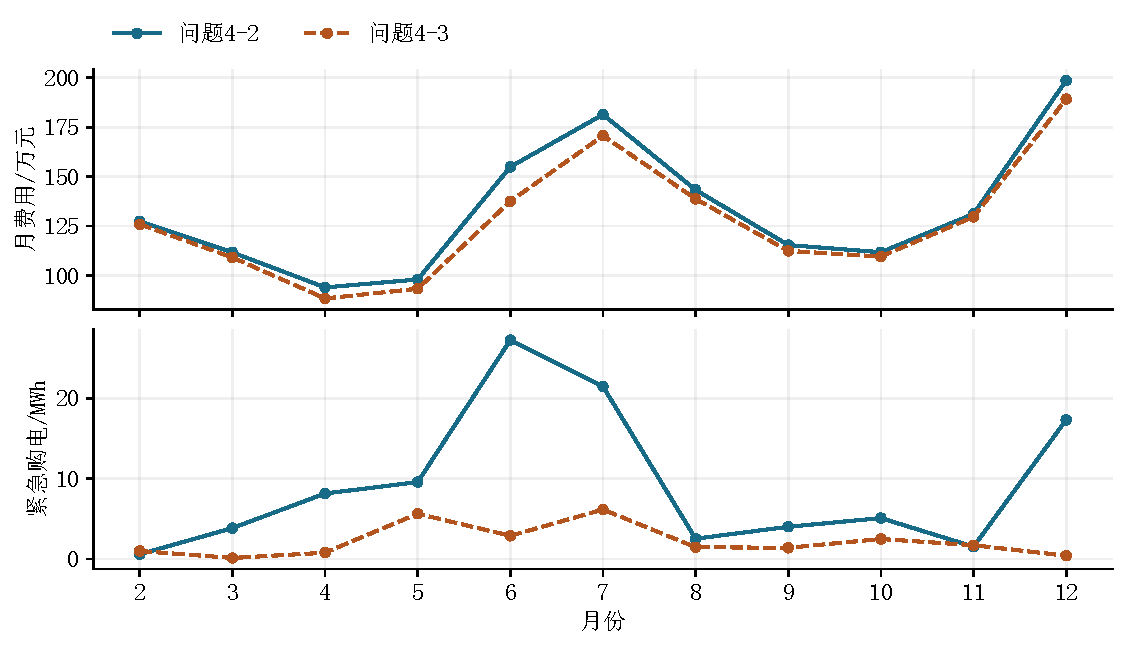
\includegraphics[width=\textwidth]{../outputs/figures/paper-q4-months.pdf}
 \caption{波动电价下各月费用与紧急购电量}\label{fig:q4-months}
\end{figure}
\FloatBarrier
指定日期费用列于表\ref{tab:q4-days-summary}。在9月23日，允许调整后的全天总费从49762.23元降至45799.34元；12月21日两种方案费用均较高。下一小节分别展示9月23日的购电与储能；其余日期、紧急事件及账单见附录\ref{app:q4-2-days}、\ref{app:q4-3-days}，完整策略保存在\texttt{result4-2.xlsx}、\texttt{result4-3.xlsx}。
\par
\begin{table}[!htbp]
\centering
\caption{波动电价下指定日期费用（2025年，元）}\label{tab:q4-days-summary}
\normalsize
\begin{tabular}{lrrr}
\toprule
\multicolumn{1}{c}{日期} & \multicolumn{1}{c}{问题4-2} & \multicolumn{1}{c}{问题4-3} & \multicolumn{1}{c}{日内方案节省} \\
\midrule
03-20 & 42,627.22 & 42,600.22 & 27.00 \\
06-21 & 19,640.47 & 18,336.05 & 1,304.42 \\
09-23 & 49,762.23 & 45,799.34 & 3,962.89 \\
12-21 & 75,769.21 & 72,885.14 & 2,884.07 \\
\bottomrule
\end{tabular}
\end{table}
\par


在共同热启动下比较光伏来源，融合方案比纯历史基准少支出122075.92元，也比单用附件三更省费，完整结果见附录\ref{app:parameter-checks}表\ref{tab:q4-3-forecast}。各预测方法分别选择参数，因此费用差反映了预测方法与相应控制参数共同作用的结果。
\FloatBarrier

\subsubsection{代表日期的购电与储能结果}
\textbf{a) 问题4-2：零时固定计划。}以下按题面表1、表2列出9月23日。购电表给出常规计划电量及按实际交付价格结算的常规费；电量为kWh，费用为元。
% Generated by scripts/build_paper_tables.py; do not edit by hand.
2025.9.23的购电和储能结果分别见表\ref{tab:q4-2-2025-09-23-purchase}和表\ref{tab:q4-2-2025-09-23-storage}。

\par
\begin{table}[!htbp]
\centering
\caption{微网在指定时间段的购电量及全天的购电量和购电费（2025.9.23）}\label{tab:q4-2-2025-09-23-purchase}
\normalsize
\begin{tabular}{lrlrlr}
\toprule
\multicolumn{1}{c}{时间段} & \multicolumn{1}{c}{购电量} & \multicolumn{1}{c}{时间段} & \multicolumn{1}{c}{购电量} & \multicolumn{1}{c}{时间段} & \multicolumn{1}{c}{购电量} \\
\midrule
10:00--10:10 & 0.00 & 12:00--12:10 & 499.87 & 14:00--14:10 & 0.00 \\
16:00--16:10 & 531.67 & 18:00--18:10 & 775.50 & 20:00--20:10 & 0.00 \\
\multicolumn{2}{c}{全天购电量} & 68,171.89 & \multicolumn{2}{c}{全天购电费} & 44,011.52 \\
\bottomrule
\end{tabular}
\end{table}
\par


\par
\begin{table}[!htbp]
\centering
\caption{储能设备在指定时间段的充放电量及0:00和24:00的储电量（2025.9.23）}\label{tab:q4-2-2025-09-23-storage}
\normalsize
\begin{tabular}{lrrlrr}
\toprule
\multicolumn{1}{c}{时间段} & \multicolumn{1}{c}{充电量} & \multicolumn{1}{c}{放电量} & \multicolumn{1}{c}{时间段} & \multicolumn{1}{c}{充电量} & \multicolumn{1}{c}{放电量} \\
\midrule
0:00--4:00 & 4,837.74 & 54.89 & 4:00--8:00 & 801.19 & 6,062.63 \\
8:00--12:00 & 5,459.91 & 1,896.62 & 12:00--16:00 & 4,418.80 & 560.16 \\
16:00--20:00 & 79.59 & 5,673.19 & 20:00--24:00 & 5,585.42 & 2,617.77 \\
\multicolumn{2}{c}{0:00储电量} & 5,901.66 & \multicolumn{2}{c}{24:00储电量} & 6,226.87 \\
\bottomrule
\end{tabular}
\end{table}
\par


\FloatBarrier

\textbf{b) 问题4-3：日内调整。}购电表分别展示零时原计划与最终常规购电，费用口径与问题三相同，均按实际交付价格核算；储能表列实际运行结果。指定日的初始库存承接前日，两组方案均从全年起点6000\,kWh连续运行至该日。
% Generated by scripts/build_paper_tables.py; do not edit by hand.
2025.9.23的购电和储能结果分别见表\ref{tab:q4-3-2025-09-23-purchase}和表\ref{tab:q4-3-2025-09-23-storage}。

\par
\begin{table}[!htbp]
\centering
\caption{微网在指定时间段的购电量及全天的购电量和购电费（2025.9.23）}\label{tab:q4-3-2025-09-23-purchase}
\normalsize
\begin{tabular}{lrlrlr}
\toprule
\multicolumn{6}{c}{零时原计划} \\
\multicolumn{1}{c}{时间段} & \multicolumn{1}{c}{购电量} & \multicolumn{1}{c}{时间段} & \multicolumn{1}{c}{购电量} & \multicolumn{1}{c}{时间段} & \multicolumn{1}{c}{购电量} \\
\midrule
10:00--10:10 & 0.00 & 12:00--12:10 & 401.83 & 14:00--14:10 & 0.00 \\
16:00--16:10 & 520.87 & 18:00--18:10 & 763.88 & 20:00--20:10 & 0.00 \\
\multicolumn{2}{c}{全天购电量} & 65,294.82 & \multicolumn{2}{c}{全天购电费} & 42,202.79 \\
\addlinespace
\multicolumn{6}{c}{最终常规购电} \\
时间段 & 购电量 & 时间段 & 购电量 & 时间段 & 购电量 \\
10:00--10:10 & 0.00 & 12:00--12:10 & 401.83 & 14:00--14:10 & 0.00 \\
16:00--16:10 & 520.87 & 18:00--18:10 & 793.71 & 20:00--20:10 & 0.00 \\
\multicolumn{2}{c}{全天购电量} & 67,099.79 & \multicolumn{2}{c}{全天购电费} & 44,903.59 \\
\bottomrule
\end{tabular}
\end{table}
\par


\par
\begin{table}[!htbp]
\centering
\caption{储能设备在指定时间段的充放电量及0:00和24:00的储电量（2025.9.23）}\label{tab:q4-3-2025-09-23-storage}
\normalsize
\begin{tabular}{lrrlrr}
\toprule
\multicolumn{1}{c}{时间段} & \multicolumn{1}{c}{充电量} & \multicolumn{1}{c}{放电量} & \multicolumn{1}{c}{时间段} & \multicolumn{1}{c}{充电量} & \multicolumn{1}{c}{放电量} \\
\midrule
0:00--4:00 & 4,267.49 & 194.62 & 4:00--8:00 & 996.54 & 6,251.03 \\
8:00--12:00 & 5,281.76 & 1,896.62 & 12:00--16:00 & 5,288.36 & 509.61 \\
16:00--20:00 & 111.95 & 5,255.66 & 20:00--24:00 & 5,591.15 & 3,287.90 \\
\multicolumn{2}{c}{0:00储电量} & 6,169.40 & \multicolumn{2}{c}{24:00储电量} & 6,224.67 \\
\bottomrule
\end{tabular}
\end{table}
\par


\FloatBarrier

\subsubsection{价格与参数灵敏度检验}
先检验预测峰谷价差的影响。记$m_{d,s}$为本次剩余时段的预测价格均值，将价格曲线改为
\begin{equation}
 \widehat p^{(s,\theta)}_{d,t}
 =\max\{0.001,m_{d,s}+(1+\theta)
       (\widehat p^{(s)}_{d,t}-m_{d,s})\},\qquad
 \theta\in\{-0.2,0,0.2\}.\label{eq:price-sensitivity}
\end{equation}
负扰动缩小预测峰谷差，正扰动扩大预测峰谷差，均根据当时可得的预测曲线计算。各组采用相同负荷、光伏、实际结算价、控制参数及1月热启动，从2月起按扰动后的预测重新规划并连续运行。表\ref{tab:q4-price-sensitivity}列出实际费用和年末库存。
\par
\begin{table}[!htbp]
\centering
\caption{预测价差幅度扰动（共同热启动，2—12月）}\label{tab:q4-price-sensitivity}
\normalsize
\begin{tabular}{lrrrr}
\toprule
\multicolumn{1}{c}{方案} & \multicolumn{1}{c}{$\theta$} & \multicolumn{1}{c}{总费用/元} & \multicolumn{1}{c}{较主方案增费/元} & \multicolumn{1}{c}{期末储电量/kWh} \\
\midrule
问题4-2 & -0.2 & 14,674,479.32 & -1,365.55 & 6,263.02 \\
问题4-2 & 0 & 14,675,844.87 & 0.00 & 6,263.02 \\
问题4-2 & +0.2 & 14,683,290.13 & 7,445.26 & 6,263.02 \\
问题4-3 & -0.2 & 14,042,823.76 & -2,061.48 & 5,997.11 \\
问题4-3 & 0 & 14,044,885.25 & 0.00 & 5,997.11 \\
问题4-3 & +0.2 & 14,061,149.66 & 16,264.42 & 5,997.11 \\
\bottomrule
\end{tabular}
\end{table}
\par

\FloatBarrier
扩大预测价差20\%时，两种策略分别增费7445.26元和16264.42元；缩小20\%时分别减费1365.55元和2061.48元。四组扰动与各自主方案的期末库存相同，可在相同储备水平下比较支出。本次范围内总费变化均小于0.12\%，日内调整方案仍更省费。该检验说明策略对价差幅度的小范围变化较稳定，峰谷时刻错位和极端电价的影响仍待检验。

另作已知未来价格的对照，直接用实际价格规划，问题4-2与4-3费用分别为\PaperValue{q4-2-oracle}\,元和\PaperValue{q4-3-oracle}\,元。该对照使用了执行时无法提前获得的信息，热启动和后续库存也随之变化，因此仅作为事后参考，尚不足以给出随机全年问题的严格下界。实际预测策略的零时平均绝对价格误差约为0.04456元/kWh，其费用影响需结合购电量和储能动作分析。

风险参数的选择结果见附录\ref{app:parameter-checks}表\ref{tab:q4-calibration}。按1月15—31日费用评分，问题4-3固定融合权重0.50，固定计划和日内调整分别在0.80和0.65处取得候选中的最低费用。提高分位可减少缺口，也会增加提前购电支出；这里的选择仅依据1月评分。
\FloatBarrier
跨月实验按训练先于评价的顺序\upcite{cerqueira2020evaluation}，每月根据上月费用重选参数，各组从共同4月1日库存连续运行。问题4-3的逐月选参方案比固定参数多支出16320.66元，9个月中仅1个月更省，说明频繁重选在本年度没有改善累计费用。完整账单与库存见附录\ref{sec:rolling}。

在相同信息、参数及热启动条件下，将储能控制换成确定性滚动反馈\upcite{wytock2017dem}，问题4-2和4-3分别增费33995.79元、213489.58元，期末库存与原反馈相同。该配置尚未估计跨日库存价值，结果说明它在本组设置下未优于原反馈；进一步改进需同时考虑次日的用电需求。模型及费用分解见附录\ref{sec:feedback}。
\label{end:q4}


\input{sections/forecast}
\section{问题三与四：日内信息更新和购电调整}
\subsection{小时光伏预报的因果融合}
在00、06、12、18点发布预报后，只接收此时及此前已发布的附件三记录。发布时刻$h$后的第$k$个小时预报对应绝对目标$h+k$，不能把不同发布行的第$k$列当成同一时刻。插值以最近一个已完成区间的光伏观测为当前锚点，连接可用的未来整点值，生成十分钟预测$\widehat P^{V,F}$；首日无历史锚点取0。到当日24点即截断。

为平衡历史稳定性与预报更新，构造
\begin{equation}
 \widehat P^V=(1-\lambda)\widehat P^{V,H}+\lambda\widehat P^{V,F},
 \qquad\lambda\in\{0,0.25,0.50,0.75,1\}.\label{eq:fusion}
\end{equation}
日内发布时刻$s\in\{36,72,108\}$，用已经完成的最近18段更新负荷水平：
\begin{equation}
 \widehat P^{L,(s)}_{d,t}=\widehat P^L_{d,t}\,
 \operatorname{clip}\!\left(
 \frac{\overline{P^L_{d,s-18:s}}}{\max(\overline{\widehat P^L_{d,s-18:s}},1)},0.75,1.25\right),\quad t\ge s.
\end{equation}
横线上标区间表示该区间均值，$\operatorname{clip}$将比例限制在给定范围。所有更新都排除当前未完成区间及之后的真实数据。

将5个权重与6个分位组成30个候选，仍只用1月15—31日费用选参。表\ref{tab:jan-selection}对每个权重列出其最优分位，问题三和问题4-3均选择$(\lambda,\alpha)=(0.50,0.65)$。实际主策略的1月热启动固定为纯附件三、0.80分位和三次日内调整，2月1日才切换参数。候选回放与正式热启动是两条明确分开的流程。
% Generated by scripts/build_paper_tables.py; do not edit by hand.
\par
\begin{table}[!htbp]
\centering
\caption{各光伏融合权重下的1月最优分位候选}\label{tab:jan-selection}
\normalsize
\begin{tabular}{lrrrr}
\toprule
\multicolumn{1}{c}{$\lambda$} & \multicolumn{1}{c}{问题3的$\alpha$} & \multicolumn{1}{c}{验证费（元）} & \multicolumn{1}{c}{问题4-3的$\alpha$} & \multicolumn{1}{c}{验证费（元）} \\
\midrule
0 & 0.65 & 857,322.99 & 0.65 & 962,646.48 \\
0.25 & 0.65 & 852,752.88 & 0.65 & 957,788.58 \\
0.5 & 0.65 & 852,457.19 & 0.65 & 957,308.74 \\
0.75 & 0.65 & 855,178.07 & 0.65 & 961,388.59 \\
1 & 0.65 & 860,734.61 & 0.65 & 968,141.26 \\
\bottomrule
\end{tabular}
\end{table}
\par


\subsection{主合约下的日内重规划}
题目给出了增购、减购和紧急电的加价，但对多次调整的累计方式存在解释空间。本文主合约按同一交付段相对零时计划的最终净调整收费：
\begin{equation}
 C_3=\sum_{d,t}\left[p_tg_{d,t}+1.5p_t\pos{q_{d,t}-g_{d,t}}
       +0.5p_t\pos{g_{d,t}-q_{d,t}}+5p_te_{d,t}\right].\label{eq:netbill}
\end{equation}
原计划款不退款。该解释把未交付增购视为可撤回的计划申报，尚未交付时可以重新改报；并非所有交易市场都采用这一规则。

在免费不利用余电的模型中，把某段$q_t<g_t$提高至$g_t$、相应增加未利用量，可以保持储能轨迹并免去减购服务费，因此不减购原计划具有弱优势。日内时刻$s$只优化$t\ge s$，以当前实际$S_s$为起点，解
\begin{equation}
 \min\sum_{t=s}^{143}1.5\widehat p_t(q_t-g_t),\qquad
 q_t\ge g_t,\quad S_{144}\ge6000,\label{eq:replan}
\end{equation}
并满足风险净负荷下的物理约束。已交付段保持不变。由于基准始终为$g_t$，新计划可低于此前尚未交付的增购申报；最终只在交付时按式\eqref{eq:netbill}收取一次调整费。问题三使用已知固定价格，问题4-3使用下述因果价格预测。

\subsection{问题四的未知价格与统一执行流程}
在波动价格情形，将历史价格按负荷相同的同星期规则加权得到$\overline p_{d,t}$；不足一周时使用衰减0.8的近期日均。首日各发布时间均沿用附件一固定价格，不作日内比例修正。对$d\ge1$，零时取$\widehat p_{d,t}=\max(\overline p_{d,t},0.001)$；日内更新为
\begin{equation}
 \widehat p^{(s)}_{d,t}=\max\left\{0.001,\overline p_{d,t}\,
 \operatorname{clip}\!\left(
 \frac{\overline{p_{d,s-18:s}}}{\max(\overline{\overline p_{d,s-18:s}},0.01)},0.5,1.5\right)\right\},\quad t\ge s.
\end{equation}
式中内层$\overline p$是历史价格曲线，外层横线为最近18段均值。问题4-2与问题二有相同决策频率，仅在零时形成价格预测；问题4-3允许三次日内更新。两种情况下，计划用$\widehat p$优化，而账单用交付时已经实现的$p$逐段重算。问题4-2选择$\alpha=0.80$，问题4-3采用上述融合参数。

统一运行流程如下：
\begin{enumerate}
 \item 零时继承真实库存，构建只含可用历史的负荷、光伏及价格预测，计算风险净负荷并生成原计划。
 \item 对每个十分钟段，若其起点是允许的发布时间，先读取已发布预报和已完成区间观测，以当前实际库存重规划剩余常规购电。
 \item 在交付段实际需求到达后，执行充放电反馈和必要的紧急购电，计算本段电费并更新库存。
 \item 日末将真实库存原样传递至次日。1月用于初始化和选参，2月起累计正式账单。
\end{enumerate}
离线预先计算预测数组只用于加速，任何决策取数仍受日期及发布时间约束。因果检查通过改变尚未发生的实测或尚未发布的预报，验证当前决策的输入不变。
\FloatBarrier

\section{主结果与信息价值分析}
\subsection{四种策略的费用、电量和库存}
正式评价期为2025年2月1日至12月31日，共334天。表\ref{tab:core-costs}将原计划、调整和紧急费用分别列示；表\ref{tab:core-energy}与表\ref{tab:core-storage}提供常规电量、未利用电量、储能吞吐量及期初期末库存。
% Generated by scripts/build_paper_tables.py; do not edit by hand.
\par
\begin{table}[!htbp]
\centering
\caption{四种主方案的正式期费用（2025年2—12月，元）}\label{tab:core-costs}
\normalsize
\begin{tabular}{lrrrr}
\toprule
\multicolumn{1}{c}{方案} & \multicolumn{1}{c}{原计划费用} & \multicolumn{1}{c}{调整费用} & \multicolumn{1}{c}{紧急费用} & \multicolumn{1}{c}{总费用} \\
\midrule
问题2 & 13,291,625.72 & 0.00 & 616,550.23 & 13,908,175.95 \\
问题3 & 12,649,467.17 & 527,937.93 & 138,430.89 & 13,315,835.99 \\
问题4-2 & 14,032,328.84 & 0.00 & 643,516.03 & 14,675,844.87 \\
问题4-3 & 13,366,608.69 & 550,605.94 & 127,670.62 & 14,044,885.25 \\
\bottomrule
\end{tabular}
\end{table}
\par

% Generated by scripts/build_paper_tables.py; do not edit by hand.
\par
\begin{table}[htbp]
\centering
\caption{四种主方案的正式期电量与库存（kWh）}\label{tab:core-energy}
\footnotesize
\setlength{\tabcolsep}{4pt}
\renewcommand{\arraystretch}{1.15}
\begin{tabular}{lrrrrr}
\toprule
方案 & 最终常规购电 & 紧急购电 & 未利用电量 & 期初储电量 & 期末储电量 \\
\midrule
问题2 & 21,712,548.31 & 102,787.48 & 2,646,069.43 & 6,840.33 & 6,258.37 \\
问题3 & 21,197,074.02 & 25,862.57 & 2,021,445.81 & 7,089.87 & 5,987.72 \\
问题4-2 & 21,708,087.29 & 101,425.76 & 2,632,806.82 & 6,864.27 & 6,263.02 \\
问题4-3 & 21,192,613.91 & 24,227.41 & 2,009,834.69 & 7,114.54 & 5,997.11 \\
\bottomrule
\end{tabular}
\par\smallskip
\begin{minipage}{0.97\linewidth}\footnotesize 期初为2月1日00:00；期末为12月31日24:00。未利用电量包括弃光和不接收的已付费常规购电。\end{minipage}
\end{table}
\par

% Generated by scripts/build_paper_tables.py; do not edit by hand.
\par
\begin{table}[!htbp]
\centering
\caption{四种主方案的原计划购电与储能吞吐量（2—12月，kWh）}\label{tab:core-storage}
\normalsize
\begin{tabular}{lrrr}
\toprule
\multicolumn{1}{c}{方案} & \multicolumn{1}{c}{原计划购电量} & \multicolumn{1}{c}{充电输入} & \multicolumn{1}{c}{放电输出} \\
\midrule
问题2 & 21,712,548.31 & 6,476,845.40 & 5,246,768.54 \\
问题3 & 20,755,552.37 & 6,648,911.63 & 5,386,610.35 \\
问题4-2 & 21,708,087.29 & 6,516,094.01 & 5,278,577.27 \\
问题4-3 & 20,752,288.47 & 6,678,014.81 & 5,410,197.68 \\
\bottomrule
\end{tabular}
\end{table}
\par

固定价格下，允许日内调整的主方案较无调整方案节省\PaperValue{q3-saving}\,元，降幅\PaperValue{q3-saving-percent}\%；波动价格下节省\PaperValue{q4-3-saving}\,元，降幅\PaperValue{q4-3-saving-percent}\%。紧急电量和紧急费用均明显下降，但常规电和库存路径也随策略而变。这些差值是完整政策组合的比较，不能全部解释为新预报本身的价值。

主方案在每段均满足供需和储能约束。期初库存是连续热启动得到的真实值，并非强制6000\,kWh；年末库存也无免费补足。各方案的起止库存均明确报告，评价现金支出时没有再按某个主观价格折算库存。问题三与其历史预测基准、反馈对照采用相同期初库存，便于控制比较条件。

\begin{figure}[htbp]
 \centering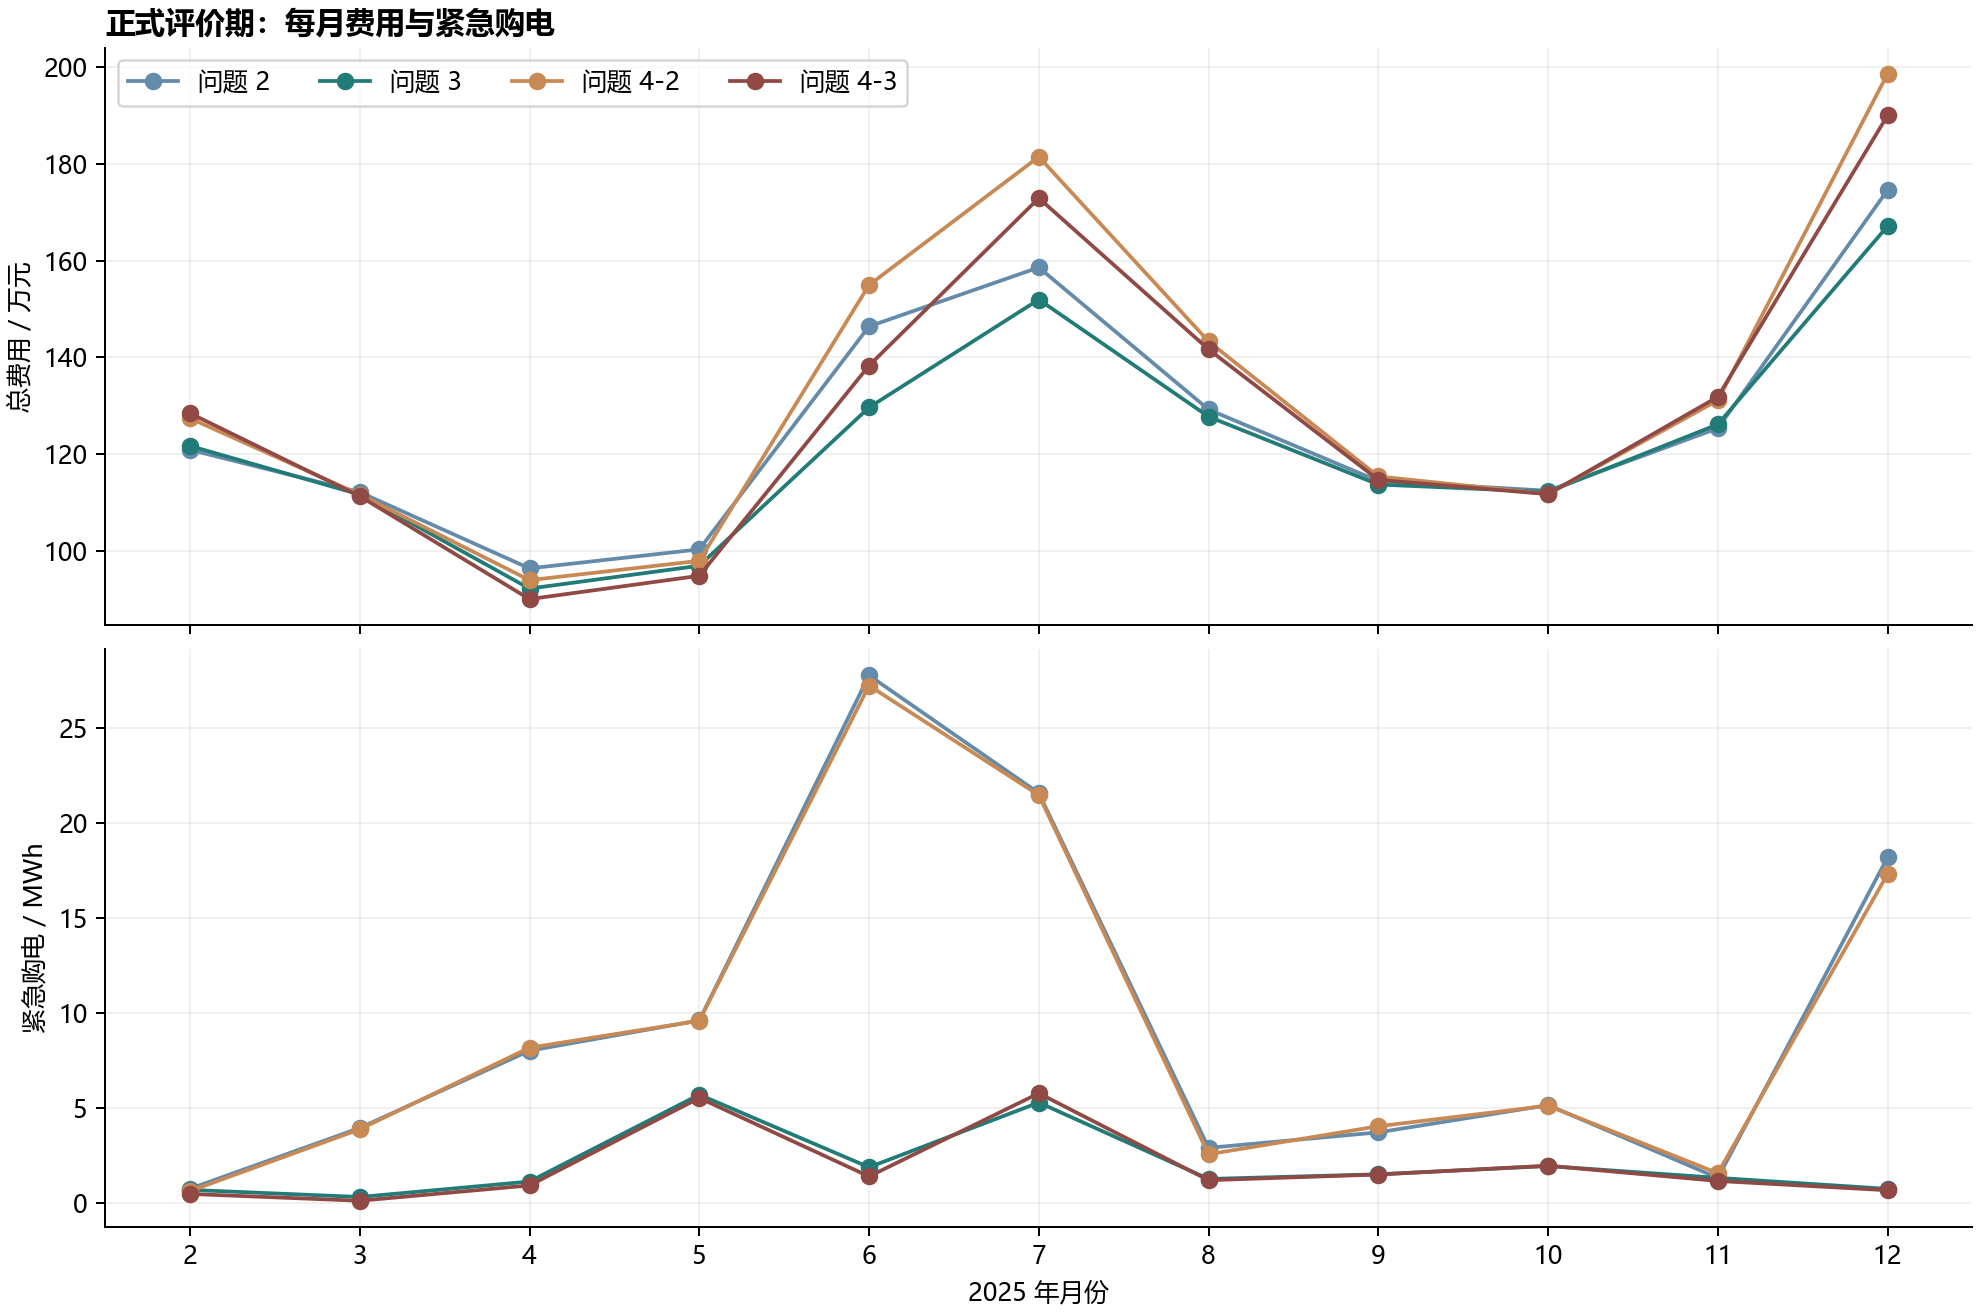
\includegraphics[width=\textwidth]{../outputs/figures/monthly-comparison.png}
 \caption{四种主方案在正式期各月的总购电费用与紧急购电量}\label{fig:monthly}
\end{figure}
3月20日、6月21日、9月23日、12月21日的指定购电时段、四小时充放电、全天费用与紧急事件完整列于附录\ref{app:days}。日内方案同时列原计划与最终常规购电；最终常规购电不含紧急电。不能将原计划费与“原计划费加调整费”再次相加。
\FloatBarrier

\subsection{历史光伏与纯附件三基准}
仅证明带日内调整的方案优于问题二不足以说明预测器有效。为此对纯历史光伏、纯附件三及两者融合均按相同1月评分区间选参，并用共同热启动比较正式期费用。
% Generated by scripts/build_paper_tables.py; do not edit by hand.
\par
\begin{table}[htbp]
\centering
\caption{共同热启动下的预测策略比较（2—12月）}\label{tab:forecast-baselines}
\small
\setlength{\tabcolsep}{4pt}
\renewcommand{\arraystretch}{1.15}
\begin{tabular}{lrrrrr}
\toprule
方案 & 光伏预测 & $\lambda$ & $\alpha$ & 费用（元） & 紧急电（kWh） \\
\midrule
问题3 & 纯附件3 & 1 & 0.65 & 13,511,208.12 & 21,565.68 \\
问题3 & 纯历史 & 0 & 0.65 & 13,428,215.91 & 38,224.16 \\
问题3 & 融合主方案 & 0.5 & 0.65 & 13,315,835.99 & 25,862.57 \\
问题4-3 & 纯附件3 & 1 & 0.65 & 14,258,363.92 & 20,483.78 \\
问题4-3 & 纯历史 & 0 & 0.65 & 14,166,961.16 & 38,253.28 \\
问题4-3 & 融合主方案 & 0.5 & 0.65 & 14,044,885.25 & 24,227.41 \\
\bottomrule
\end{tabular}
\par\smallskip
\begin{minipage}{0.97\linewidth}\footnotesize 各问题内的比较共用1月热启动及正式期初库存。各预测器依据同一1月准则选参，费用差是策略组合之差。\end{minipage}
\end{table}
\par

融合主方案相对共同热启动的历史基准，在问题三节省112379.91元，在问题4-3节省122075.92元；纯附件三在本数据上反而更贵。由此采用融合而非完全依赖附件三。但上述差值比较了经选参的预测与控制组合，仍包含风险残差和后续库存轨迹变化。

\subsection{新增小时光伏预报的严格子集对照}
为隔离新增小时预报，固定主预测器参数、规划器和反馈规则，保留06、12、18点三次重规划、当时真实库存、负荷修正及当前光伏观测锚点，仅改变允许读取的新小时预报集合。未读取时沿用最近可用发布行，并按相同绝对目标整点对齐。每种信息集合独立构造因果残差并连续运行。表中直接列出允许读取的新预报时刻，融合策略各子集共用1月热启动；纯附件三列用于展示原预测器下的同类对照。
% Generated by scripts/build_paper_tables.py; do not edit by hand.
\par
\begin{table}[htbp]
\centering
\caption{问题3新小时光伏预报的完整子集对照}\label{tab:hourly-subsets}
\small
\setlength{\tabcolsep}{4pt}
\renewcommand{\arraystretch}{1.15}
\begin{tabular}{lrrr}
\toprule
新增预报时刻 & 纯附件3费用（元） & 融合策略费用（元） & 融合紧急电（kWh） \\
\midrule
无 & 13,580,285.75 & 13,333,061.82 & 29,178.88 \\
18 & 13,580,285.30 & 13,333,062.82 & 29,178.86 \\
12 & 13,564,801.30 & 13,344,238.23 & 29,324.32 \\
12、18 & 13,564,801.43 & 13,344,238.54 & 29,324.42 \\
06 & 13,585,837.75 & 13,335,964.19 & 25,744.14 \\
06、18 & 13,585,837.09 & 13,335,963.52 & 25,744.09 \\
06、12 & 13,511,207.99 & 13,315,835.68 & 25,862.47 \\
06、12、18 & 13,511,208.12 & 13,315,835.99 & 25,862.57 \\
\bottomrule
\end{tabular}
\par\smallskip
\begin{minipage}{0.97\linewidth}\footnotesize 各行均保留06、12、18点重规划、实际SOC、负载修正及当前光伏观测锚点；仅开关新小时预报。融合子集共用1月热启动。\end{minipage}
\end{table}
\par

全部允许相对全部不读取，正式费用减少17225.82元。分别从完整集合去掉06点、12点或18点新小时预报，费用变化为$+28402.55$元、$+20127.52$元与$-0.31$元。这些边际量有交互作用，不能直接求和；18点的量级不能支持可辨认的经济增益。

若连重规划机会一并取消，会同时失去调整库存、修正负荷和提前增购的能力。允许全部重规划相对仅零时规划的费用差为745563.95元，属于整体策略效果。故“18点新光伏预报没有可辨认的改善”不等于“18点调整购电没有价值”。
\FloatBarrier

\input{sections/discussion}
\FloatBarrier
\clearpage

\bibliographystyle{gbt7714-numeric}
\bibliography{references}
\clearpage
\appendix
\section{程序与支撑文件索引}\label{app:support}
题面要求的完整日期结果与关键对照已列于正文。表\ref{tab:support-files}给出程序和完整数据的入口；运行环境及命令见支撑材料README。
\begin{table}[!htbp]
 \centering
 \caption{主要程序与支撑文件}\label{tab:support-files}
 \begin{tabular}{lp{0.41\textwidth}}
  \toprule
  \multicolumn{1}{c}{文件或目录} & \multicolumn{1}{c}{用途} \\
  \midrule
  \path{scripts/prepare_data.py} & 原始附件对齐与审计 \\
  \path{scripts/model.py} & 预测、规划、反馈与费用结算 \\
  \path{scripts/solve.py} & 主策略求解入口 \\
  \path{scripts/evaluate_round2.py} & 反馈对照与逐月选参实验 \\
  \path{scripts/validate_results.py} & 主调度物理及费用独立核验 \\
  \path{scripts/validate_round2.py} & 补充对照独立核验 \\
  \path{scripts/build_paper_tables.py} & 由归档生成并核对论文表格 \\
  \path{outputs/deliverables/} & 五份题目要求的完整Excel \\
  \path{outputs/main/} & 十分钟主调度及费用归档 \\
  \path{outputs/experiments/revision/} & 完整选参、预报子集与合约结果 \\
  \path{outputs/experiments/round2/} & 逐月参数、费用差额及反馈路径 \\
  \bottomrule
 \end{tabular}
\end{table}
\FloatBarrier

\end{document}
